\subsection{Application: Medical Image Classification}

Medical image classification is a high-consequence application in which the foundations of machine learning become operational requirements rather than abstract principles. Dataset partitioning must prevent patient or study leakage, representation choices determine which anatomical structures are retained, class imbalance changes the interpretation of accuracy, and decision thresholds must be selected using validation data rather than tuned on the final test set. A strong benchmark therefore reports both discrimination and thresholded error behavior.

This application uses chest radiography to connect those foundational ideas to a compact, reproducible image-classification problem. The experiment is deliberately lightweight: instead of introducing a large convolutional architecture that belongs in the later deep-learning and computer-vision chapters, it compares conventional feature representations and classifiers on a standardized public benchmark. This keeps the focus on the Chapter 1 questions of hypothesis class, representation, validation, threshold selection, and generalization.

The dataset is PneumoniaMNIST from MedMNIST, a standardized chest-X-ray benchmark with official train, validation, and test splits. The validation partition is used to select the operating threshold for each model, and the test partition is used only for final evaluation. This separation makes the benchmark a direct example of the validation discipline developed earlier in the chapter.

\\textbf{Problem:} The task is binary classification of pediatric chest radiographs as normal or pneumonia. The statistical objective is to learn a score that ranks pneumonia cases above normal cases while preserving a clinically interpretable tradeoff between sensitivity and false-positive burden. The benchmark is educational and is not intended to support clinical deployment.

\\textbf{Dataset:} PneumoniaMNIST contains 5,856 grayscale chest-X-ray images standardized to \(28\times 28\) pixels. The official split contains 4,708 training images, 524 validation images, and 624 test images. The labels are binary: normal versus pneumonia. The experiment preserves these predefined splits rather than randomly repartitioning the data.

\\textbf{Model:} Three classical baselines are compared. Pixel logistic regression uses the standardized image intensities directly, providing a linear hypothesis over the pixel space. HOG logistic regression replaces raw pixels with histogram-of-oriented-gradient features, introducing an explicit edge and local-shape representation before the same linear classifier. A class-balanced random forest provides a nonlinear baseline on the flattened image intensities.

\\textbf{Method:} Each model is fit only on the training split. The validation split is used to select the probability threshold that maximizes F1 for that model, and the selected threshold is then frozen before evaluating the test set. Pixel and HOG logistic regression use standardized features; the HOG representation is computed with fixed cells, blocks, and orientation bins. The random forest uses fixed random seed 1729 and class balancing.

\\textbf{Evaluation:} ROC--AUC and average precision summarize threshold-independent ranking behavior. Accuracy, precision, recall, and F1 are reported at the validation-selected threshold. Figure~\ref{fig:ch1-medical-pneumonia} links representation and evaluation: panels (a) and (b) show the test-set mean normal and pneumonia radiographs, while panel (c) reports the test precision--recall curves. Table~\ref{tab:ch1-medical-pneumonia-benchmark} provides the reproduced numerical comparison.

\begin{figure}[t]
\centering
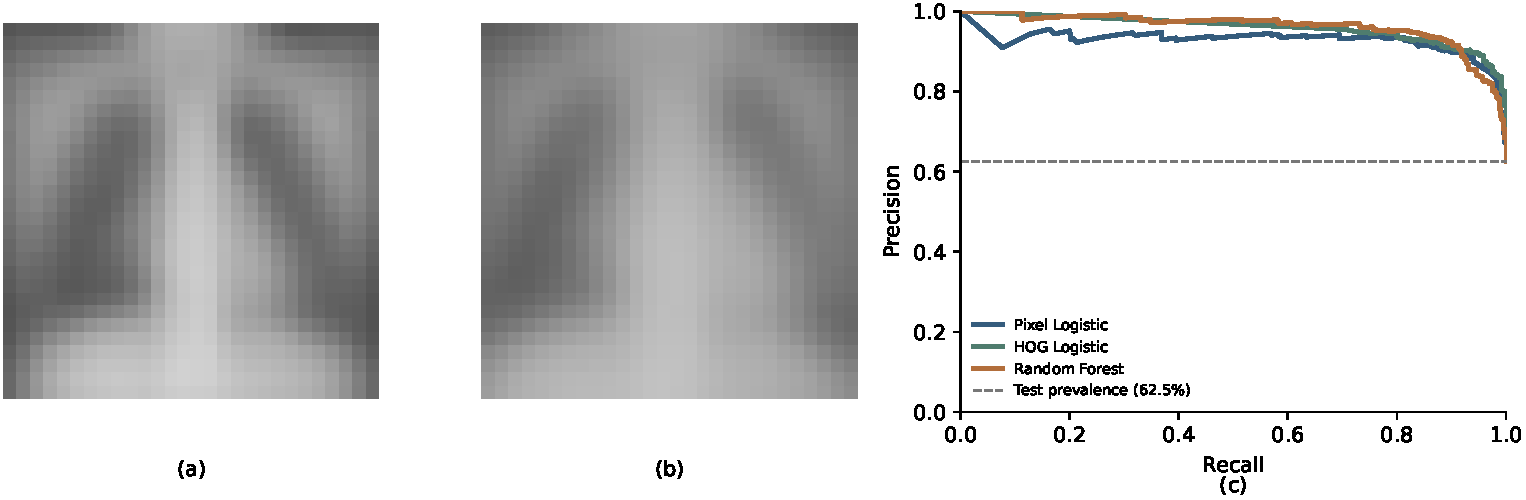
\includegraphics[width=\BookFigureWidth]{figures/ch01_medical_pneumoniamnist.pdf}
\caption{Reproduced PneumoniaMNIST benchmark for Chapter 1 medical-image classification. (a) Mean test image for the normal class. (b) Mean test image for the pneumonia class. These class-average images summarize broad intensity and anatomical differences without implying diagnostic localization. (c) Test precision--recall curves for pixel logistic regression, HOG logistic regression, and a class-balanced random forest, together with the positive-class prevalence. Thresholds used for the tabulated precision, recall, and F1 values are selected on the separate validation split rather than on the test set.}
\label{fig:ch1-medical-pneumonia}
\end{figure}

\begin{table}[t]
\centering
\small
\caption{Reproduced PneumoniaMNIST test-set comparison using the official train, validation, and test partitions. Thresholded metrics use the threshold selected on the validation split.}
\label{tab:ch1-medical-pneumonia-benchmark}
\begin{tabular}{lrrrrrr}
\toprule
Model & ROC--AUC & AP & Accuracy & F1 & Precision & Recall \\
\midrule
Pixel logistic & 0.9224 & 0.9255 & 0.8381 & 0.8838 & 0.8017 & 0.9846 \\
HOG logistic & 0.9393 & 0.9432 & 0.8429 & 0.8879 & 0.8017 & 0.9949 \\
Random forest & 0.9437 & 0.9612 & 0.8333 & 0.8802 & 0.7992 & 0.9795 \\
\bottomrule
\end{tabular}
\end{table}

\\textbf{Results:} The HOG representation improves both ROC--AUC and average precision relative to raw-pixel logistic regression, showing that a representation aligned with local edge structure can improve a simple linear hypothesis class. The random forest achieves the strongest ranking metrics, with ROC--AUC of 0.9437 and average precision of 0.9612, while the HOG logistic model produces the strongest F1 among the three baselines. All three validation-selected thresholds emphasize high recall, which is consistent with the asymmetric cost of missing a positive case in a screening-style setting.

\\textbf{Error Analysis:} A high recall value does not by itself establish clinical usefulness. False positives increase downstream review burden, and false negatives require direct inspection for image quality, subtle findings, acquisition artifacts, and representation failures. Because the images are standardized to \(28\times 28\), fine radiographic detail is deliberately compressed; errors can therefore arise from resolution limits as well as from the classifier. A production study would also stratify errors by patient, acquisition site, demographic variables, and disease severity when those metadata are available.

\\textbf{Limitations:} PneumoniaMNIST is a small educational benchmark derived from pediatric chest radiographs and is not intended for clinical use. The images are downsampled substantially, and the benchmark does not establish external generalization to other hospitals, scanners, age groups, or disease prevalence. The experiment also uses classical models rather than modern high-resolution medical-imaging architectures because the purpose in Chapter 1 is to isolate foundational questions of representation and validation.

\\textbf{Deployment / Engineering Implications:} The key Foundations lesson is that medical-image performance depends on the complete experimental protocol. Patient-level separation, external validation, calibration, prevalence-aware metrics, and a clinically defined threshold are necessary before a model can support decision making. A high test AUROC is not sufficient if the split leaks patient identity, the threshold is tuned on the test set, or the predicted probabilities are poorly calibrated for the deployment population.
